\chapter{Architecture Evolution}
\label{ch:evolution}

This chapter describes how the target architecture defined in Part~1 evolved during implementation. It covers what remained unchanged, what was refined, and what was cut.

\section{What Remained Unchanged}

The five bounded contexts identified in Part~1 held through implementation without revision:

\begin{enumerate}
    \item \textbf{Catalog:} inside nopCommerce; owns product definitions, pricing, categories.
    \item \textbf{Order Management:} inside nopCommerce; owns the order lifecycle, customer intent, payment authorisation.
    \item \textbf{Identity:} inside nopCommerce (cross-cutting); owns customer accounts and authentication.
    \item \textbf{Inventory / Warehouse:} extracted; owns authoritative stock truth, reservations, stock movements.
    \item \textbf{Shipping / Fulfillment:} extracted; owns carrier dispatch, tracking, delivery state.
\end{enumerate}

The \textbf{transactional outbox} as the reliability mechanism was also confirmed and not revisited. The feasibility spike (Part~1, \S7) had already de-risked the critical constraint: \texttt{PlaceOrderAsync} does not run inside an ambient \texttt{TransactionScope}, so the outbox decorator must supply one.

\section{Structural Change: Two Plugins Instead of One}

Part~1 described a single plugin (\texttt{Nop.Plugin.Misc.OmnichannelOutbox}) carrying both the outbox write and the inbound RabbitMQ subscriber. During implementation, the inbound side was split into a \textbf{separate plugin}: \texttt{Nop.Plugin.Misc.OmnichannelConsumers}.

\begin{table}[H]
\centering
\caption{Plugin split rationale}
\label{tab:plugin-split}
\begin{tabularx}{\textwidth}{@{} L{4.5cm} X @{}}
\toprule
\textbf{Plugin} & \textbf{Responsibility} \\
\midrule
\texttt{OmnichannelOutbox} & Outbox write path: entity, publisher decorator, dispatcher, RabbitMQ publisher, TransactionScope decorator, retention cleanup \\
\addlinespace
\texttt{OmnichannelConsumers} & Inbound path: RabbitMQ subscriber, inbox deduplication, event handlers, compensation orchestration \\
\bottomrule
\end{tabularx}
\end{table}

This separation follows the single-responsibility principle at plugin granularity and mirrors the Part~1 ADD iteration structure (Iteration~1 = outbox, Iteration~2 = consumers and stock projection).

\section{New: \texttt{Compensated} Order State}

The \texttt{Compensated} state was added to the \texttt{OrderStatus} enum in \texttt{Nop.Core}. This was anticipated in Part~1 but is now concrete code. The state is reached when the Inventory service rejects a stock reservation and the compensation flow (payment release, customer notification) completes.

\begin{figure}[H]
\centering
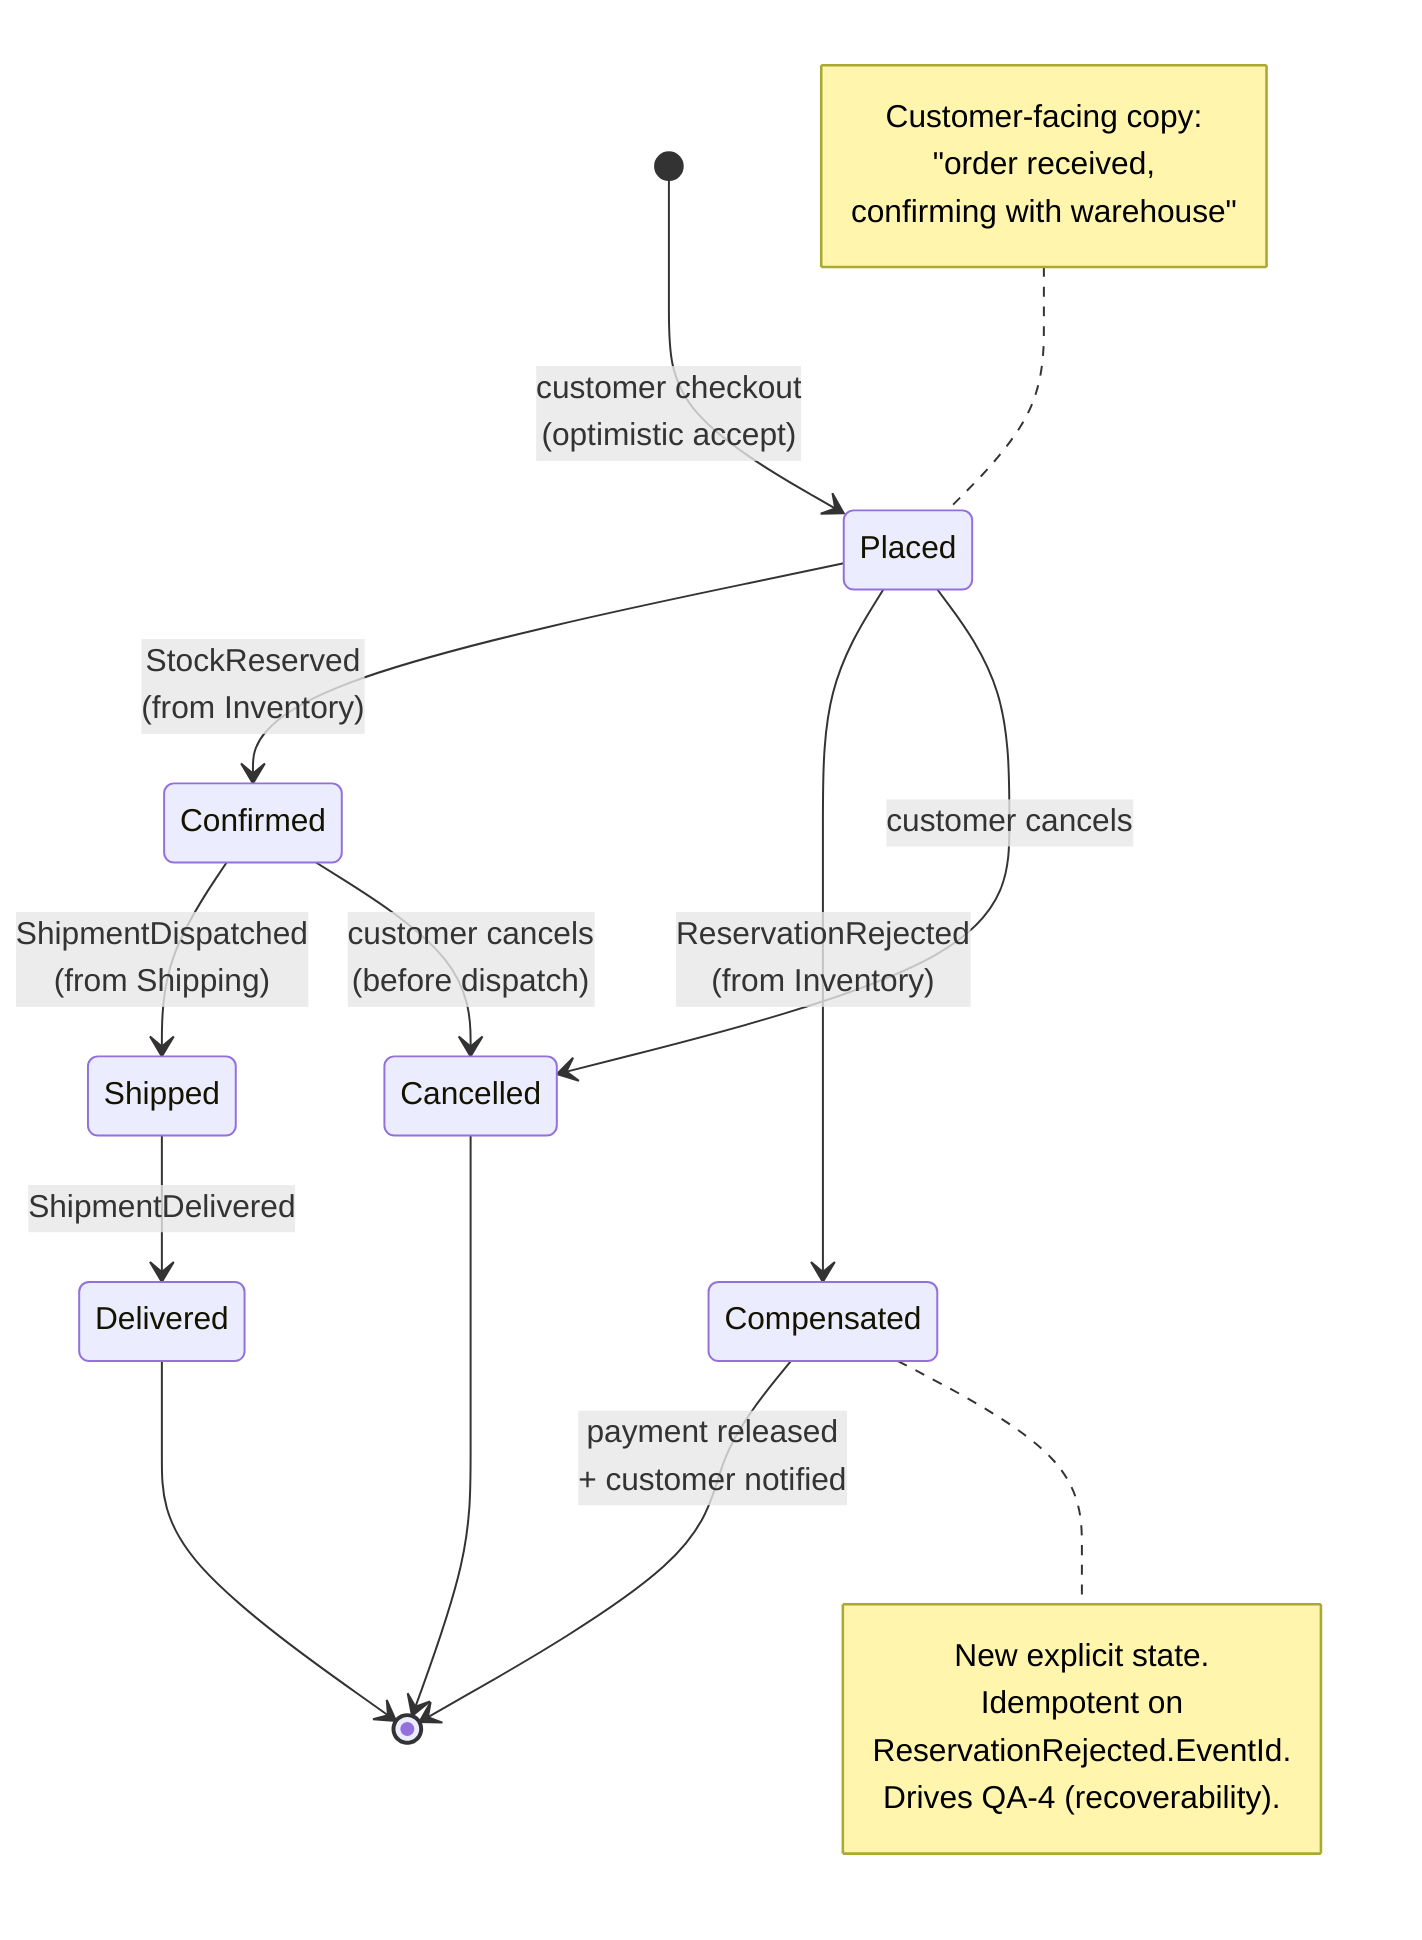
\includegraphics[width=\textwidth]{figures/order-lifecycle.png}
\caption{Order lifecycle state machine including the new \texttt{Compensated} state}
\label{fig:order-lifecycle}
\end{figure}

\section{New: Inbox Deduplication}

Part~1 stated that consumers must be idempotent but left the mechanism open. The implementation chose an \textbf{inbox table} approach: a \texttt{ProcessedInboxMessage} entity records every \texttt{EventId} that has been handled. Before processing any inbound message, \texttt{InboxDeduplicationService} checks for an existing record. Duplicates are silently discarded.

This satisfies the at-least-once delivery guarantee without requiring exactly-once semantics from RabbitMQ.

\section{Event Contracts Settled}

The event contracts were implemented as dedicated event classes in \texttt{Nop.Core.Domain}:

\begin{table}[H]
\centering
\caption{Cross-context event contracts}
\label{tab:events}
\begin{tabularx}{\textwidth}{@{} L{5cm} L{2.5cm} X @{}}
\toprule
\textbf{Event} & \textbf{Direction} & \textbf{Published when} \\
\midrule
\texttt{OrderPlacedEvent} & Outbound & Customer places an order \\
\texttt{StockReservedEvent} & Inbound & Inventory confirms stock reservation \\
\texttt{Reservation\-Rejected\-Event} & Inbound & Inventory cannot fulfil the reservation \\
\texttt{OrderConfirmedEvent} & Outbound & Order moves to \texttt{Confirmed} state \\
\texttt{StockLevelChangedEvent} & Inbound & External stock movement \\
\texttt{ShipmentDispatchedEvent} & Inbound & Shipping service dispatches the parcel \\
\texttt{OrderCompensatedEvent} & Internal & Compensation flow completes \\
\bottomrule
\end{tabularx}
\end{table}

\section{Scope Cuts Carried Over From Part~1}

All acknowledged scope cuts from Part~1 remain in force:

\begin{scopebox}
\begin{itemize}
    \item Identity stays as-is (no federated SSO across channels).
    \item Payment is folded into Order Management, with no separate Payment service.
    \item Shipping equals Fulfillment: one extracted service, not two.
    \item Single nopCommerce instance: no Redis, no horizontal scaling.
    \item The outbox lives \textbf{inside the monolith process} as an \texttt{IScheduleTask}, not as a separate worker.
\end{itemize}
\end{scopebox}
